
\section{Kleinian Groups}
クライン群について学習する際には書籍『インドラの真珠』\cite{indra}を読むことを勧める.インドラの真珠は数学者以外にもクライン群の魅力を伝えるために書かれた.中には研究者レベルの高度な内容も出てくるが,高校レベルの数学と簡単なプログラムを組む能力があれば,自分で図をレンダリングしながら読み進めることができるだろう.
この章では,クライン群に関する用語を確認した後にレンダリング手法と『インドラの真珠』では言及のないクライン群の話題を紹介する.

\subsection{Group}
まず,群という語はここでは変換の集まりだと考えることにする.例えば,図のような二種類の変換を考えてみよう.逆変換の4種類の変換を組み合わせることで,たくさんの変換を作ることができる.これらの変換すべての集合を群と呼ぶこととする.クライン群はメビウス変換を生成元にもつ群のなかで離散性という性質を持つものをいう.
またここでは変換にラベルを付けて扱う.変換を小文字のアルファベットで表し,その逆変換を大文字で綴る.
ラベルを並べて書くことで,変換の合成を表す.その際に右側の変換から使うことに注意する.
例えば点pに対してaabaという変換を用いると,pを右上右右の順で点を動かすことになる.
また,上付文字はその変換の無限列とする.例えば,$\overline{a}$としたとき,$aaaaa...$といった変換$a$の無限列となる.通常これはどの点に適用しても変換$a$の固定点に収束する.


\subsection{M\"obius Transformations}
メビウス変換は一次分数変換とも呼ばれ,以下のように表現される.
\begin{eqnarray*}
 a, b, c, d\in \mathbb{C}, f(z) = \frac{az + b}{cz + d}
\end{eqnarray*}
我々がなじみ深い平行移動,拡縮や回転といった操作もメビウス変換に含まれる.
これを2×2の複素数行列として扱うことで,変換の合成を行列の積とすることができる.
\begin{eqnarray*}
  A = \left(
    \begin{array}{ccc}
      a & b \\
      c & d
    \end{array}
  \right)
\end{eqnarray*}
メビウス変換は複素数平面上に作用し,等角性や円円対応といった性質をもつ.
図\ref{fig:circleInversion}はメビウス変換の中でも重要な役割を持つ,円に関する反転という操作を可視化したものである.
それぞれの図形は黒い円に関する反転で移されている.緑色の矩形を観察すると,変換の前後で直角が保たれていることがわかる.また,黄色の円は円が保たれている.メビウス変換は角度は保つが形は大きく歪めてしまう.
\begin{figure}[htbp]
 \begin{center}
      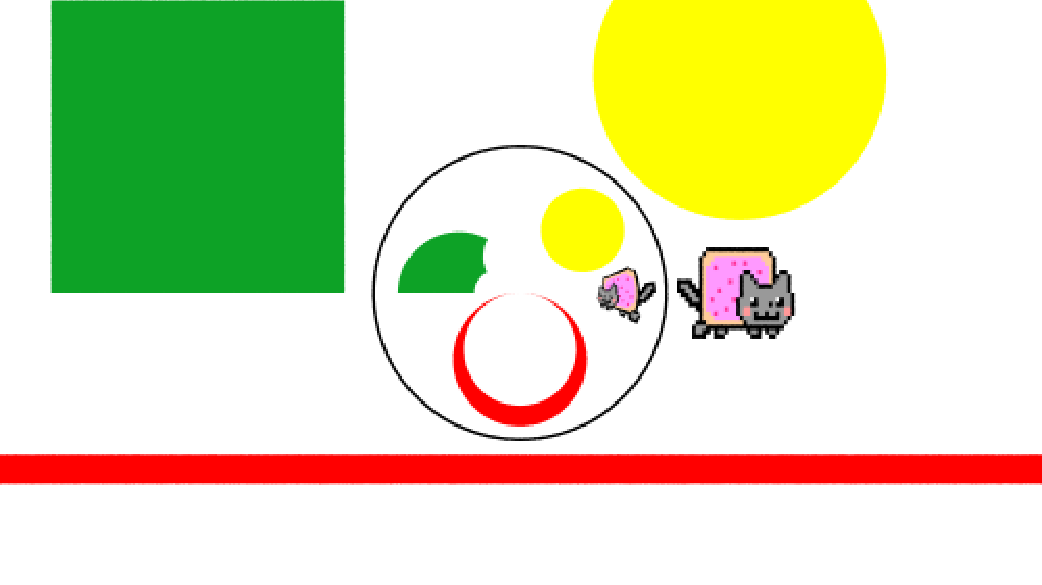
\includegraphics[width=3in, height=3in, keepaspectratio]{../img/klein/circleInversion.pdf}
    \caption{Circle Inversion}
    \label{fig:circleInversion}
 \end{center}
\end{figure}

メビウス変換は固定点の個数で分類することができる.固定点とは,$f(z) = z$となるような,メビウス変換を使って動かすことのできない点である.複素平面上の点はメビウス変換を繰り返し適用することで固定点へと収束していく.
固定点が2個の場合を斜航型変換,固定点が1個の場合を放物型変換,固定点がない場合を楕円型変換と呼ぶ.また斜航型変換の中でも,その係数が正の実数である時,その変換を双曲型変換と呼ぶ場合もある.
クライン群の描画において,メビウス変換の分類は重要である.なぜならば,多くの楕円型変換を含む群はクライン群にはなりえない.また,放物型変換は固定点への収束が遅いという特徴をもつ.これは後述する極限集合の描画の際に考慮することとなる.

メビウス変換は4つの複素数で構成されていることから,8つのパラメータがある.ただし,このままでは自由度が高すぎるため,適切に制限を加えた群の「レシピ」が作られている.
『インドラの真珠』で使われる「おばあちゃんのレシピ」をみてみよう.
パラメータは二つの複素数と符合となった.綺麗な図が描けるように調整されている.

\subsection{Graph Traversal Approach}

群を構成する変換の全組み合わせを調べるとき,変換の語で構成される木構造を考える.
図のような木はケーリーグラフ(Cayley graph)と呼ばれる.
この木を幅優先探索するか,深さ優先探索するかで描画できるものが変わってくる.

\subsubsection{Rendering the Orbit of Transformations}
群を可視化する.軌道を描くことで群を可視化してみよう.
4つの円の反転を生成元に持つ群の可視化を考える.図は赤色の円を周囲の橙色の円で反転した軌道を表したものである.赤色の円は4つの円で反転されることで,橙色の円の内側に移され,4つの小円となる.逆変換4つの円の反転を新たに現れた小円にも適用する.
このことを繰り返すと,以

それぞれの円の反転は自分以外の円を自分の内側に移す.よって,それぞれの円の内側には3つの円が移され,12個の小円ができる.次に4つの円の反転を新たに表れた小円にも適用する.このことを繰り返すと,以下の画像のように,円が入れ子状につらなる図を得ることができる.これが群の生成元による軌道である.また,円列の極限を極限集合とよぶ.この極限を観察することがクライン群を研究する上で役に立つ.
このアルゴリズムは変換で構成される木構造を幅優先探索で探索することに等しい.おおまかに生成元の作用を調べることに役立つ.
この例では,軌道の元となる図形が生成元と同じであるが,その他の図形でも可能である
図はbugman123氏による作品\footnote{http://bugman123.com/Fractals/index.html}を参考に筆者が描画したものである.蝶が二つの元の作用で変換された軌道を極限集合とともに描いている.

\subsubsection{Rendering the Limit Set}
前節でみた極限集合を直接描く.主に極限集合を描く方法が使われる.
木構造を探索し,最後に固定点に対して合成した変換を適用することで極限集合の点を求めることができる.

先に述べた平行移動の例では,abABという変換は一周してもとの場所に戻ってきてしまう.同様のことがクライン群の生成元に関しても言える.効率よく描画するためには,うまくこのような元を取り除く必要がある.これを解決するためには有限オートマトンが使われる.有限オートマトンに関する数学的な事項は『Word Processing In Groups』\cite{wordProcessing}が詳しい.

先に述べたように,メビウス変換の群すべてがクライン群になるわけではない.群のレシピのパラメータの中には描画すると極限集合が収束せず,図が乱れるようなものがある.このような群は非離散群と呼ばれ,クライン群ではない.離散と非離散の境界近くでは極限集合が興味深い形になる.この離散と非離散のパラメータ領域を表す図はスライスと呼ばれる.図はマスキットスライスと呼ばれる.どのようなパラメータが離散的であるか,すなわちクライン群となるかを調べることがクライン群の研究テーマともなる.

\subsubsection{Faults of Graph Traversal}
グラフを探索する方法は生成元や,探索を深くするごとに指数オーダーで計算量が増えてしまう.そもそも木構造の探索は並列化が難しいため,時間がかかる.
最新のOpenCLやCUDAといったGPUを用いた並列計算プラットフォームではDynamic Parallelismという機能をサポートしている.この機能を用いることで,極限集合,軌道の並列計算を行うことが可能である.

\subsection{Iterated Inversion System}
筆者らは円や球の反転で構成される群の軌道を高速に描画するためのアルゴリズム,Iterated Inversion System (IIS)\cite{iis}を開発した.
木構造の探索により,円や球の座標と半径を直接計算するこれまでのアプローチに対して,このアルゴリズムは任意の点が属する円や球の深さを特定する.
このアルゴリズムはスクリーンスペースのピクセルそれぞれに対して独立に計算することができるのでGLSLによる並列計算,描画を行うことができる.
また,Distance Estimationとレイマーチングを用いて三次元形状に関しても高速で描画することができる.

\subsection{Geometrical Representation of Mobius Transformations}

木構造を用いて群を可視化する際には,変換を行列で考えたが,行列表現でメビウス変換を操作することは直観が得にくい.さらに,四次元クライン群を構成する三次元空間に作用するメビウス変換は,2×2四元数行列で表現することができるが,さらにパラメータ数が増大する.このことは,四次元クライン群の研究があまり進んでいないことの原因にもなっている.
そこで筆者らはすべてのメビウス変換を円や球の反転で構成することを考えた.円や球を用いることで,生成元と可視化される図形の間の関係性が理解しやすく,幾何学的な直観を得ることができる.それに加え,IISを用いることで複雑な生成元をもつ群もリアルタイムに可視化することができる.このことは,研究者や学習者だけでなく,フラクタルアーティストにも有益なものとなるだろう.具体的な構成方法などはBridges2017に投稿中である.
また,筆者は円や球の反転で構成される群をインタラクティブに構成するソフトウェア,{\it Schottky Link} \footnote{Schottky LinkL: https://schottky.jp}を開発している.

\subsection{Other Topics}

\subsubsection{Other Rendering Methods}
Aaron Montag氏はIterated Inversion Systemを拡張したHyperbolic Iterated Function Systemによって極限集合を描画することに成功した\cite{hyperbolicIFS}.固定点付近では図に乱れが出るものの,おおむね描画できる.

また,Jos Ley, Knighty両氏はマスキット群におけるDistance Estimationのアルゴリズムを開発した.\footnote{An escape time algorithm for Kleinian group limit sets http://www.fractalforums.com/3d-fractal-generation/an-escape-tim-algorithm-for-kleinian-group-limit-sets/}二次元の極限集合だけでなく,三次元の群も高速に描画することができる.群は二つの放物型変換による群で,片方の元は平行移動を表す.荒木・糸\cite{maskit}による設定をうまく活用している.

\subsubsection{Quasi Fuchsian 3-Dimensional Fractals}
阿原・荒木両氏による擬フックス群を三次元に拡張した4次元クライン群である\cite{sphairahedra}\cite{sphairahedraJa}.球面体をその周囲の球で反転させていくことにより得ることができる.その極限集合は球の和集合となる.前述の三次元フラクタルのレンダリングに大きな影響を与えた.
荒木氏はこのフラクタル図形の物質化についてもまとめている\cite{materializing}.

また,Distance EstimationのアルゴリズムがKnighty氏により開発された.\footnote{Another 3D Kleinian http://www.fractalforums.com/ifs-iterated-function-systems/another-3d-kleinian/}
蔭山氏が2016年にまとめている\cite{kageyama}.

\subsubsection{4-Dimensional Kleinian Groups}
インドラの真珠で紹介されるクライン群は複素平面にのみ作用する.
四元数を用いることで,三次元空間に作用するメビウス変換を定義することができる.
これは$sp^k(1, 1)$と呼ばれ,2x2の四元数行列で表現される.
パラメータが多くなりすぎるため,あまり研究は進んでいない.
四元数で構成されるメビウス変換とその分類は佐久川氏による\cite{sakugawaMaster}や\cite{accidentalParabolic}にまとまっている.佐久川氏は,三次元空間上で捩じりが加わるようなメビウス変換を{\it Compund Parabolic},{\it Compound Loxodromic}と分類した.また,群のレシピも作られてはいるが,離散条件やスライスの描画に追試験が必要である.

荒木・糸両氏はマスキット群を四次元クライン群に拡張した\cite{maskit}.幾何学的性質をうまく使うことで,四元数の計算を避けている.レンダリングされた極限集合は糸氏のWebページ\footnote{http://www.math.nagoya-u.ac.jp/~itoken/3d-maskit/3d-maskit.html}にて見ることができる.佐久川氏はこの群の四元数表示を導出した\cite{sakugawa4d}.

三浦氏は3つ以上の生成元による4次元クライン群をモジュラー群から構成することを試みた\cite{miura}.筆者はこの論文における数値実験と可視化を行った.

\subsubsection{Once Punctured Torus Groups}
Once Punctured Torus Groupsはクライン群の一種である.OPTi\footnote{OPTi http://delta-mat.ist.osaka-u.ac.jp/OPTi/index.html}という描画ソフトウェアが有名である.
描画や離散性判定のためのアルゴリズムが和田氏によりまとめられている.
ベアズスライスとよばれる.OPTiでは,ベアズスライスも同時に描画される.
ほとんどが解決された.

\subsection{Further Readings}
この章の最後に,クライン群のより数学的な背景を学習するための書籍をいくつか挙げておく.『双曲幾何学への招待』\cite{invitation}は絶版であるが双曲幾何学の基本事項がよくまとまっている.『双曲多様体とクライン群』\cite{manifold}『Outer Circles』\cite{outerCircles}『Spaces of Kleinian Groups』\cite{space}